\chapter{Introduction}
\label{ch:Introduction}
Throughout the history of software engineering, much effort has been put on the description and understanding of high-level software processes. The waterfall model, the very first software process, has contributed to the success of many large software systems. High-level software processes divide the software development process into phases, where each phase lasts from a few days to several months \cite{Pfleeger:01,Pressman:03}. For example, the requirements analysis phase may last months before the design phase starts. Recently, increasing effort has been put on low-level software processes \cite{Larman:03,AgileAlliance}, in which a phase may last from several minutes to a few hours only. Each phase defines how developers and the development team should carry on the work on a daily basis. The Personal Software Process (PSP) \cite{Humphrey:99} and Extreme Programming (XP) \cite{Jeffries:00,Beck:00,XP96} are two examples of a low-level software process. Although proven to be useful in improving software quality\cite{Ferguson:97,Kamatar:00,MicrosoftTSP,Janzen:05}, low-level software processes are hard to execute correctly and repeatedly. Low-level software processes have the potential to require new skills from software organizations, project managers, and software developers. For example, in Test-Driven Development (TDD), each developer is a requirements analyst, designer, tester, and coder. As a result, a low-level software process could be used differently in different software organizations. Worse yet, an organization might think they are using a particular low-level process, such as TDD, but in reality, they are doing something quite different. In order to improve the quality on practice and research of low-level software processes, it would be helpful to have tools to support the understanding of what low-level software processes are actually being performed by organizations, and what the impact of these processes are on the outcome of development. In my dissertation research, I focused on one low-level software process called Test-Driven Development (TDD) \cite{Beck:03}, and developed the Zorro software system to study it.

\section{Test-Driven Development}
``Clean code that works''\cite{Beck:03} is the goal of Test-Driven Development. To achieve this goal, TDD summarizes its low-level software development process as two basic rules: ``(1) Write new code only if an automated test has failed; (2) Eliminate duplication.''  Kent Beck, the pioneer of Test-Driven Development, stated that there is an implicit order to software development using TDD \cite{Beck:03}: 
\begin{enumerate}
\item Red - Write a little test that does not work, and perhaps does not even compile at first.
\item Green - Make the test work quickly, committing whatever sins are necessary in the process.
\item Refactor - Eliminate all the duplication created by merely getting the test to work.
\end{enumerate}

The red/green/refactor order is a pithy summary of TDD. In reality, TDD is significantly more complicated than that. Given a requirement, a TDD developer analyzes it and outlines a To-Do list with a few tasks. After picking a task from the To-Do list, the developer immediately writes a test, which is then used to motivate the implementation of actual system. If the test fails, the developer does whatever is necessary to make it pass as quickly as possible, not worrying about the quality or generality of the results. Only after getting the test case to pass does the developer perform a pass over the code base to improve its quality without changing its functionality. This is called the ``refactoring'' phase. Then the developer crosses out this task from the To-Do list, and adds new tasks to it if new requirements occur to him. 

Because a test is always created first to drive the design and implementation, TDD used to be called Test-First Design (TFD) or Test-First Development (TFD). My opinion is that ``test first'' is better than ``test driven'' for describing the order of test and production coding activities. Therefore, in the rest of this document, I will use ``test first'' when it is necessary to emphasize the order of programming in TDD, but there is no difference between ``test first'' and ``test driven''.

TDD is one of the innovative practices of Extreme Programming. In TDD, the software development process is iterative and incremental \cite{Larman:03}. There is only one task to accomplish in an iteration. In any particular iteration, a unit test corresponding to the task is created first, followed by production code implementation. TDD is built on the foundation of the XUnit framework \cite{XUnit}, which has been ported to more than 30 languages. Unit testing has become a defacto standard in the software industry. TDD is widely adopted by software professionals. An informal survey \cite{UnitTestingPoll:06} conducted by the Method and Survey magazine found that 46\% of the studied software organizations perform unit testing informally, 41\% of the studied organizations document their unit test cases, and 14\% of the studied organizations use the TDD approach.

\section{TDD Challenges}
At first glance, TDD might seem easy, but in fact, it is a very difficult low-level software process that requires much discipline to carry out correctly. First, software developers are not typically educated to write unit tests for the programs they develop. Therefore, in a lot of cases, software systems are not designed for easy testing. Consequently, developers often find it is hard to write testing code at all, much less write testing code prior to implementation. Second, following the red/green/refactor software development pattern requires a lot of discipline. In TDD, software developers must continuously remain in the mindset of test-first, which is initially counter-intuitive to many of them \cite{Beck:01,Wang:04}. So they often apply it differently according to their own experience level and understanding \cite{Beck:01}. Third, the best way to divide a complicated problem into a set of tasks that can be finished in short iterations is not always obvious. Perhaps as a result,the research findings on TDD's impact on software quality and developer productivity are mixed. In order to improve the TDD practices and empirical evaluations, it is necessary to measure the usage and adoption of TDD. In this section, I will first present some TDD research findings, followed by a discussion of the ``construct validity'' problem of these studies.

\subsection{Mixed TDD Research Findings}
So far, software engineering researchers have focused heavily on the important outcomes that TDD brings to software products and software developers. Both pedagogical \cite{Muller:02,Edwards:04,Geras:04,Matjaz:03,Erdogmus:05,Kaufmann:03} and industrial \cite{George:03,Maximilien:03,Bhat:06} evaluations of TDD have been conducted in the last few years. Table \ref{tab:TDDResearchWork} lists most relevant TDD research work. 
\begin{table}[htbp]
\centering
  \caption{Research Work of TDD on Software Quality and Developer Productivity}
  \begin{tabular}{|l|l|p{2.3cm}|p{4cm}|l|} \hline 
 & Investigator	& Participants	& Software Quality	& Developer Productivity \\ \hline
 & George \cite{George:03}	& 24	& TDD passed 18\% more tests & 16\% more time \\ \cline{2-5}
 & Geras \cite{Geras:04}  &  14	& TDD has the edge on quality & No impact \\ \cline{2-5}
 Industrial
 & Maximilien	\cite{Maximilien:03}  &  9	& 50\% reduction in defect density	& Minimal impact \\ \cline{2-5}
 & Williams\cite{Williams:03} &  9	& 40\% reduction in defect density	& No change \\ \cline{2-5}
 & Bhat	\cite{Bhat:06}  & 11	& 2-4 times reduction in defect density	& 35\% and 15\% more time \\ 
 
 \hline \hline
 
         & Kaufmann \cite{Kaufmann:03}	&  8	& N/A	    & 50\% improvement \\ \cline{2-5}
         & Edwards \cite{Edwards:04} & 59	& 54\% fewer defects	& N/A \\ \cline{2-5}
Academic & Erdogmus	\cite{Erdogmus:05} & 35	& No change	  & Improved productivity \\ \cline{2-5}
         & M\"{u}ller \cite{Muller:02}& 19 & Less reliable, but better reuse	& No change \\ \cline{2-5}
         & Panc\v{u}r	\cite{Matjaz:03} & 38	& No change	  & No change \\ \hline
  \end{tabular}
  \label{tab:TDDResearchWork}
\end{table}
It is interesting to note that while the industrial empirical evaluations results are often positive, on the contrary, the pedagogical evaluations results are often negative toward TDD. The industrial studies found that TDD helped to improve software quality at the cost of development time according to Table \ref{tab:TDDResearchWork}. Most pedagogical studies did not find the improvements of software quality and degradation of developer productivity. Instead, some pedagogical studies found that students as participants improved their productivity. As presented in Table \ref{tab:TDDResearchWork}, discrepancies exist among empirical research findings, and they are not trivial. Although it is commonly understandable that empirical research work can not be repeated easily, the TDD research findings are too inconsistent to discount as mere replication variability. Next, I will discuss the process conformance problem, one of the most possible reasons that contributed to the mixed results, and motivate the need to measure TDD usage and adoption. 

\subsection{Measures of TDD Usage and Adoption}
Much of the research work on TDD suffers from the threat of ``construct validity'' \cite{Wang:04} because of the what has been termed as the ``process conformance'' problem. Wang and Erdogmus defined process conformance as the ability and willingness of the subjects to follow a prescribed process. The process conformance problem of TDD can be expressed as a simple question, ``Do test-driven developers really do test-first?''  It is a question that implies two sub questions.
\begin{enumerate}
\item Do test-driven developers have the abilities to develop software in TDD?
\item Do test-driven developers develop software in TDD consistently?
\end{enumerate} 
An empirical study has the construct validity problem if the answer to the first question is not a firm ``yes'', and it has the internal validity problem if the answer to the second question is not a firm ``yes''. Unfortunately, researchers have not paid much attention to either of these validity problems in the empirical studies I mentioned in the previous section. Some researchers used pair programming \cite{George:03} and verbal confirmation \cite{Muller:02} as the process control methods, but they are not reliable sources. So process conformance is one possible explanation to the mixed research findings of TDD.

In the software industry, TDD is gradually becoming well accepted for software development \cite{UnitTestingPoll:06}. Some companies even put TDD in their job descriptions. Yet there are still problems in testability and differences in the understanding of this methodology. In \cite{Janzen:05}, Janzen and Saiedian warned that measuring the adoption of TDD is necessary. Many organizations might be using it without talking about it. Others might claim to be using TDD when in fact they are misapplying it. Worse yet, they might be advertising its use falsely. Surveys could be conducted to gauge the usage of TDD, but often only those who are much in favor or much opposed to it will respond. 

The inability to accurately characterize process conformance is harmful to TDD. Therefore, measuring the usage and adoption of TDD has become an important issue for both researchers and practitioners. However, Janzen and Saiedian \cite{Janzen:05} stated that measuring the use of a software development methodology is hard. They claimed it is so hard to do accurately that published data on the level of TDD adoption in industry is either indirect or inaccurate \cite{Janzen:05,UnitTestingPoll:06}.

Fortunately, as my initial case study demonstrates \cite{csdl2-06-02}, measuring the use of certain software development methods such as TDD is becoming feasible with the emergence of technologies such as the Hackystat system \cite{Hackystat:06,csdl2-04-11,csdl2-04-22,csdl2-03-12}, an in-process software metrics collection and analysis framework.

\begin{comment}
In addition, there are many important research questions regarding software 
development using TDD. For example, When does it pay off to use TDD, and 
when does it not pay off to use TDD? One thing is clear: these questions cannot 
be answered accurately without good software
process measurement.   
\end{comment}

\section{Proposed Solution: Zorro Software System}
In this research, I developed the Zorro software system to measure the usage of TDD with the capabilities introduced by the Hackystat system, a framework of automated software metrics collections and analyses.  Figure \ref{fig:ZorroInfrastructure} illustrates the infrastructure of the Zorro software system. Zorro is built on top of Hackystat, and it uses Hackystat's data collection and analysis services for development behavior inference of TDD. 
\begin{figure}[htbp]
  \centering
  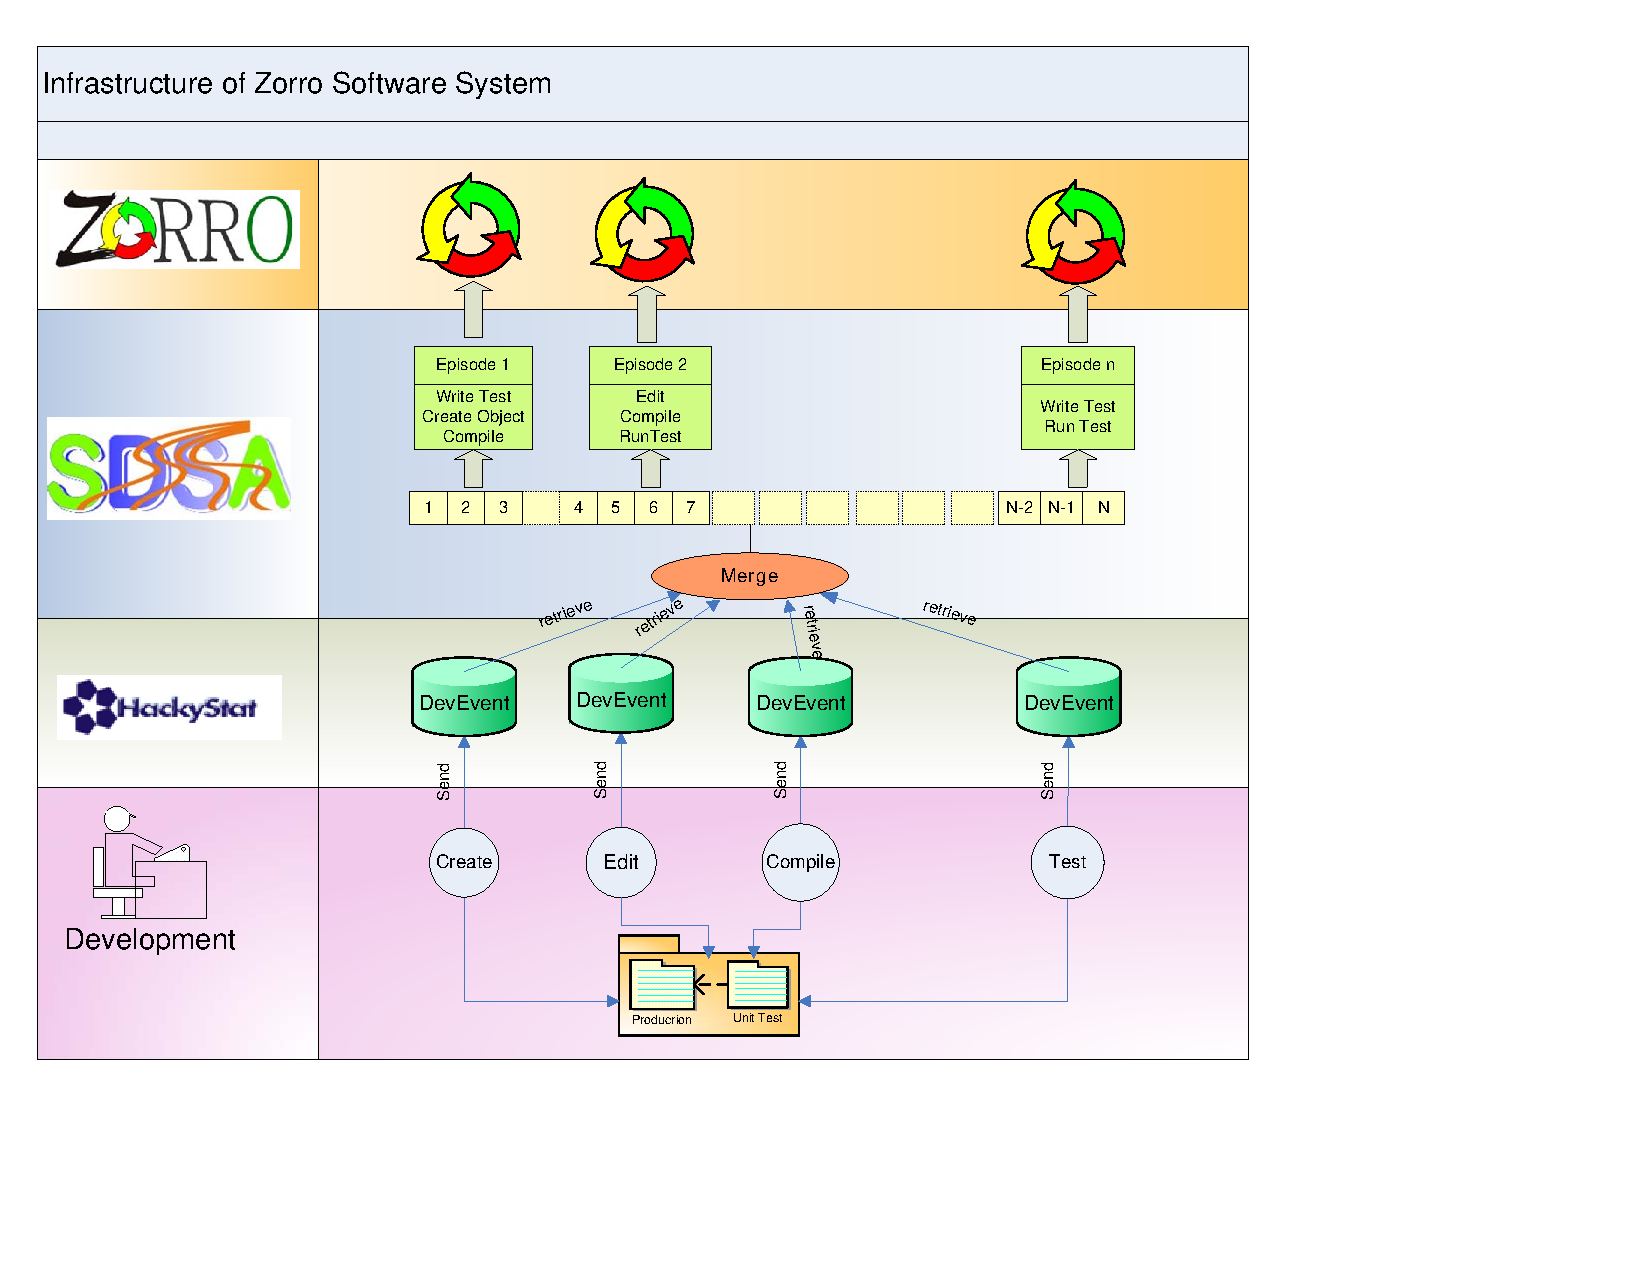
\includegraphics[width=1.0\textwidth]{figs/Visio-ZorroInfrastructure}
  \caption{Zorro Infrastructure}
  \label{fig:ZorroInfrastructure}
\end{figure}
In Figure \ref{fig:ZorroInfrastructure}, between Hackystat and Zorro layers, there is a middle tier named SDSA. The SDSA stands for the Software Development Stream Analysis, a generic framework for development event stream analysis including three components \textemdash software development stream construction, development stream partition, and development behavior inference. The SDSA is an extension of Hackystat, and it can be used to study low-level software processes.

\subsection{SDSA: A Framework of Development Stream Analysis}
The SDSA uses software metrics of development activities collected by Hackystat sensors to monitor, identify and characterize high-level development behaviors with the support of JESS \cite{Friedman-Hill:03}, a rule-based system in Java. Figure \ref{fig:Intro-SDSA-Workflow} illustrates the data models and work flow of SDSA. 
\begin{figure}[htbp]
  \centering
  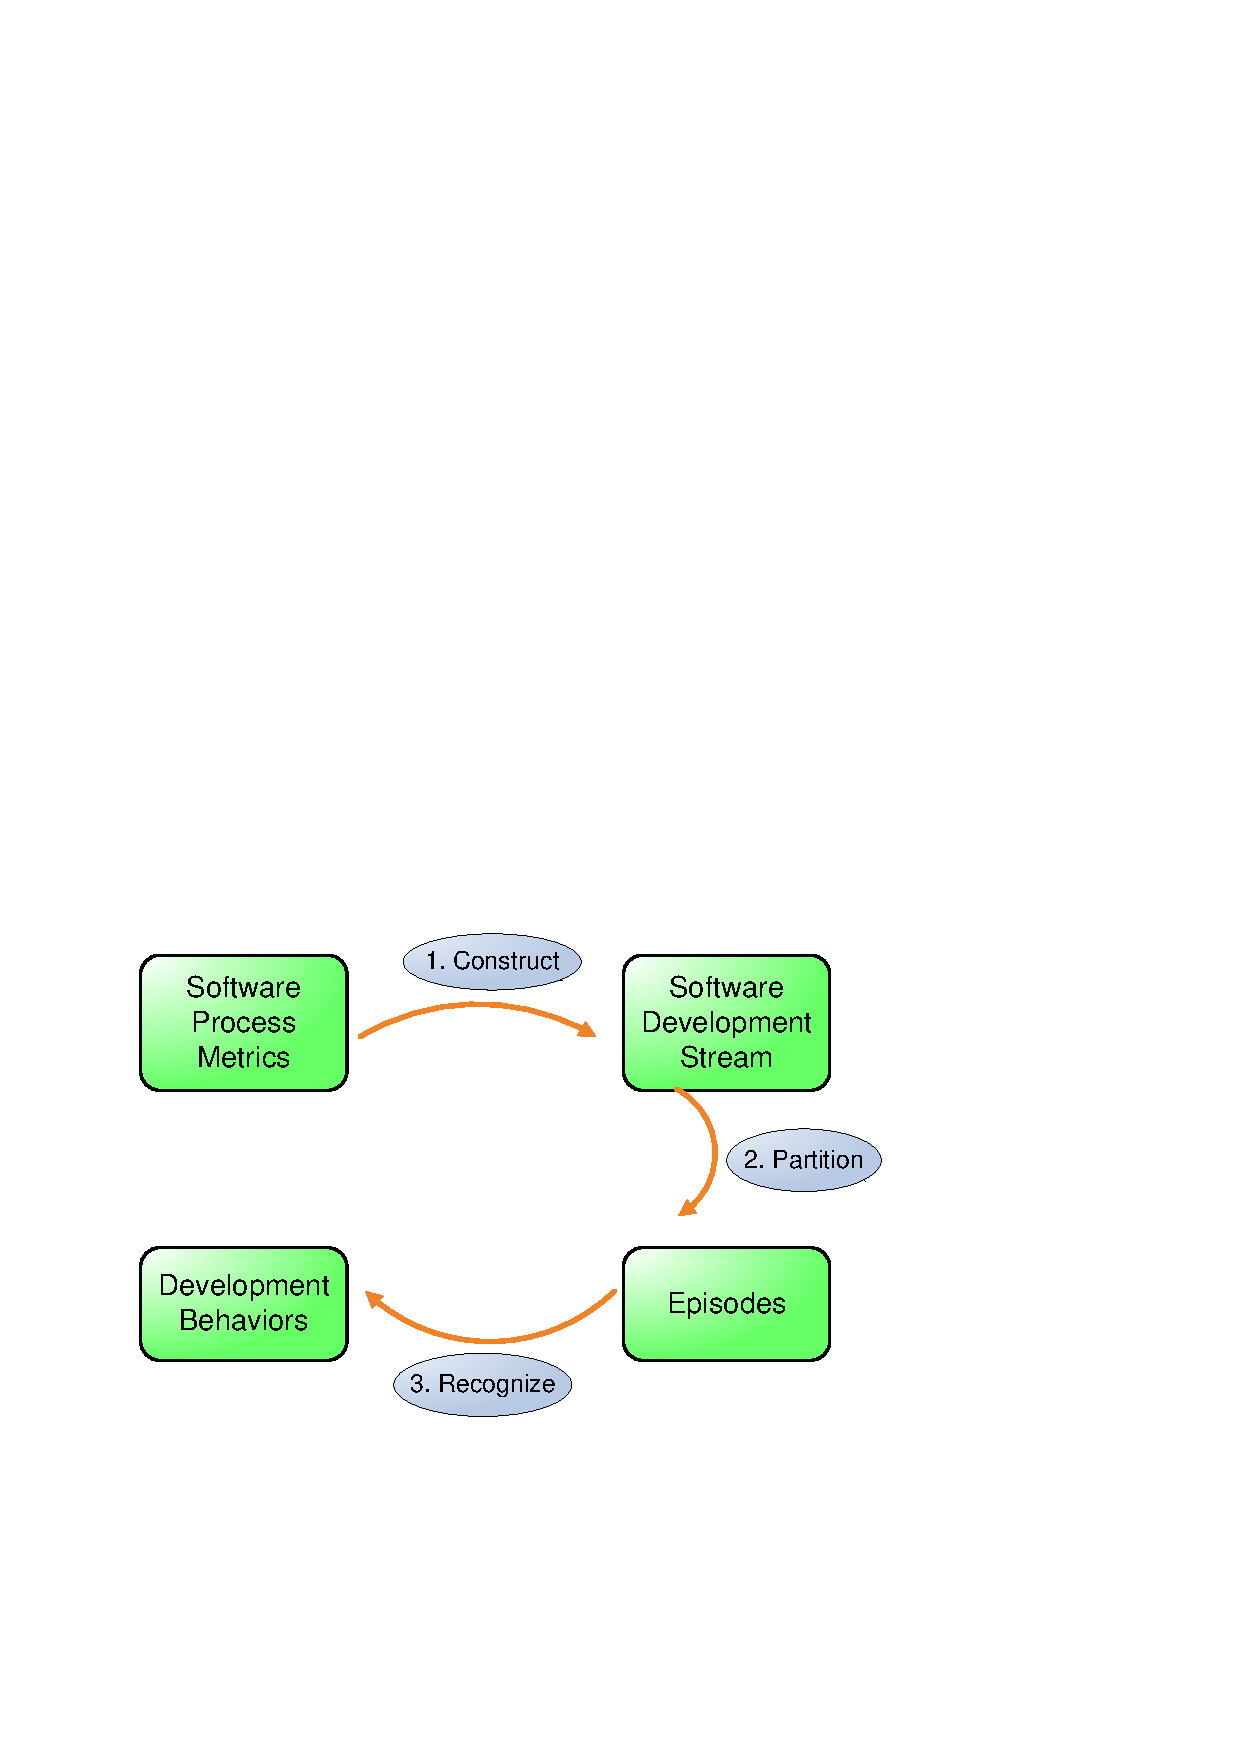
\includegraphics[width=0.5\textwidth]{figs/Visio-SDSA-FlowChart}
  \caption{SDSA Framework}
  \label{fig:Intro-SDSA-Workflow}
\end{figure}
The data models of SDSA include ``software development stream'', ``episode'', and ``development behavior''. A linear work flow connects software metrics and these three data models together in SDSA. First, SDSA processes the software metrics of development activities collected by Hackystat sensors. After reducing software process metrics into development activities, SDSA organizes development activities of a same type into a time-series event stream, which is a sub stream of the software development stream. SDSA assembles different event streams together to construct a ``software development stream'', which is also a time-series. Second, due to the complexity of digesting long development streams with heterogeneous development activities, SDSA uses a partition technique. A development stream can be partitioned into many episodes delimited by characteristic development activities. The episode is in turn a time-series collection of development activities. Third, SDSA includes a driver and interface to recognize the development behaviors in episodes using JESS. 

SDSA is tool and process independent. It can be instantiated to measure a software development method or low-level software process.

\subsection{Zorro Software System}
Zorro is an instantiation of the SDSA framework for TDD. It extends SDSA at three points: 
\begin{enumerate}
\item Development Stream Construction

As Figure \ref{fig:ZorroInfrastructure} illustrates, Hackystat sensors collect a variety of software metrics, and SDSA can construct a development stream with all of them. But this is not desirable because some development activities might not be relevant to the development method or process under study. Using TDD as an example, debugging is not interesting because it is not part of the process of TDD. In a nutshell, the essential development activities required by Zorro for TDD behavior inference are:
\begin{itemize}
\item editing activities including document, production and unit test editing,
\item buffer transition activities,
\item refactoring activities including addition, deletion, renaming, and moving of object components,     
\item unit testing activities,
\item compilation activities. 
\end{itemize}
Respectively, Zorro constructs the development streams of TDD with event streams including ``EditStream'', ``BuffTransStream'', ``RefactoringStream'', ``UnitTestStream'', and ``CompilationStream''.  

\item Tokenization

Zorro uses the ``test-pass'' tokenizer, which partitions the TDD development stream into a set of episodes that are delimited by successful unit test invocations. 

\item Development Behavior Recognition  

In Zorro, I defined a set of specific rules for TDD according to Beck \cite{Beck:01,Beck:03} and others who have described the practices of TDD. The ``test-pass'' episodes are categorized as ``test-first'', ``refactoring'', ``test-addition'', ``regression'', ``code-production'', ``test-last'', ``long'', or ``unknown''. Chapter \ref{ch:Zorro} has the detailed description of the episode classification schema. 

\end{enumerate}

After inferring development behaviors in episodes and categorizing them, Zorro uses the classification results as well as the context of episodes to reason the conformance of TDD. Figure \ref{fig:Zorro-Demo} is an excerpt of Zorro's TDD inference result for an experienced TDD developer. 
\begin{figure}[htbp]
  \centering
  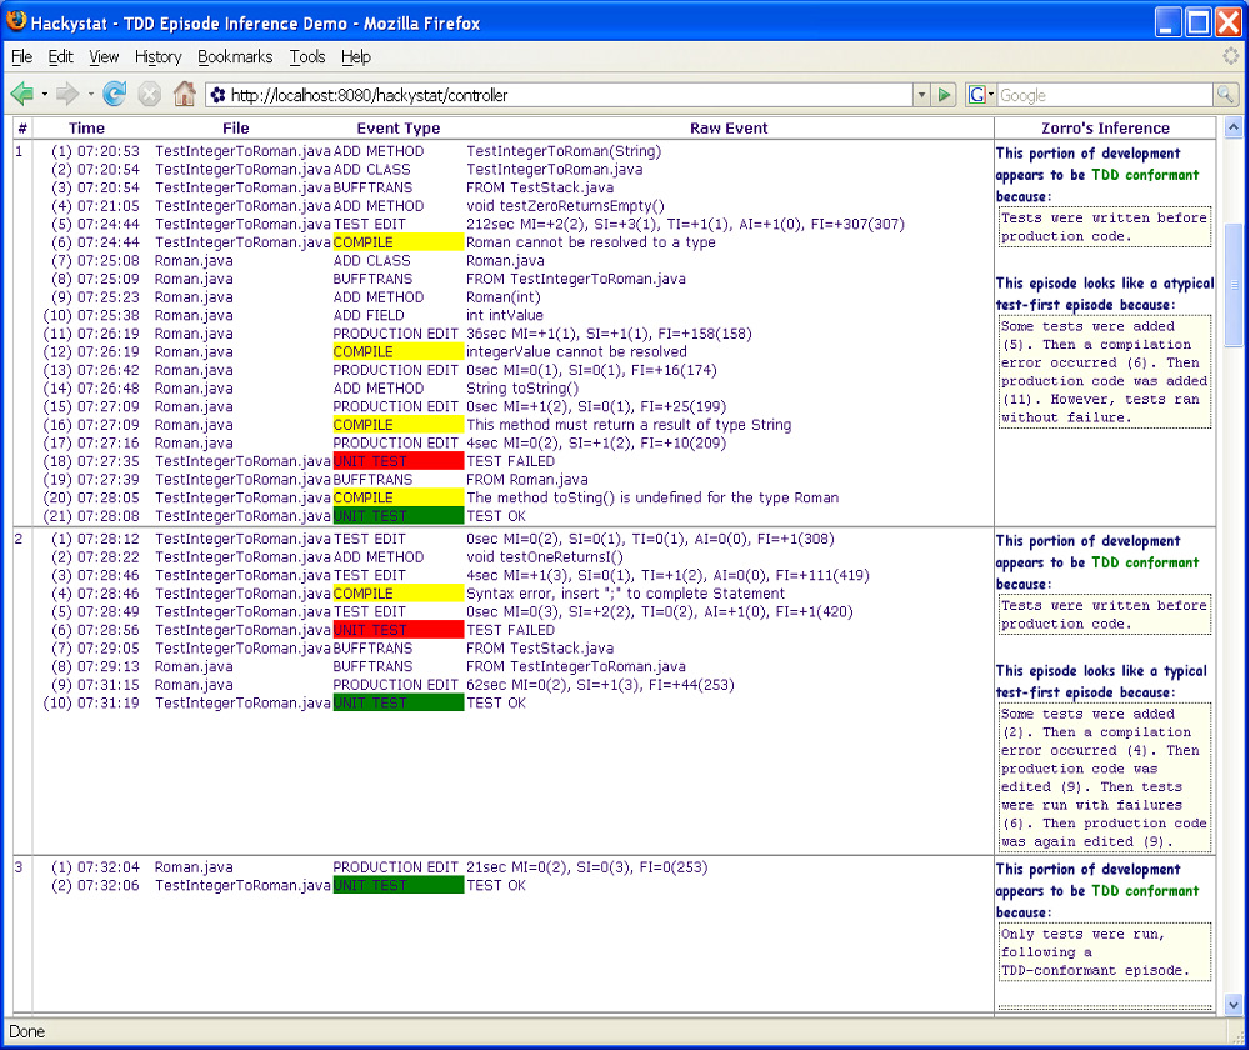
\includegraphics[width=1.0\textwidth]{figs/Zorro-Demo}
  \caption{Demo of Zorro's TDD Inference}
  \label{fig:Zorro-Demo}
\end{figure}
This experienced developer solved the Roman numeral conversion problem (Appendix \ref{app:UserStoriesRomanNumeral}) using TDD in the Eclipse IDE. The Hackystat Eclipse sensor was installed to instrument the development process to collect development activities. Zorro partitioned them into 16 episodes using the ``test-pass'' tokenizer, and inferred the process conformance of TDD.  In the table illustrated in Figure \ref{fig:Zorro-Demo}, the last column  contains the reasoning process and result. According to this table, the first three episodes are all TDD conformant. The first episode is ``test-first'' but atypical because production code was not edited to make test pass after the test invocation failed at (18). The second episode is ``test-first'' due to the perfect match of development activities to the red/green/refactor metaphor. The last episode is ``regression' because no progress was made although the production code was edited. Based upon the reasoned development behaviors and the context of episodes, Zorro inferred that all the three episodes are TDD compliant. 

With the automated software metrics collection and inference of TDD, a lot of useful analyses that once were thought impossible have become plausible. A handful of analyses (see Chapter \ref{ch:Zorro}) were implemented in Zorro. Figure \ref{fig:Zorro-Demography} illustrates one of them, the ``TDD Episode Demography'' analysis. 
\begin{figure}[htbp]
  \centering
  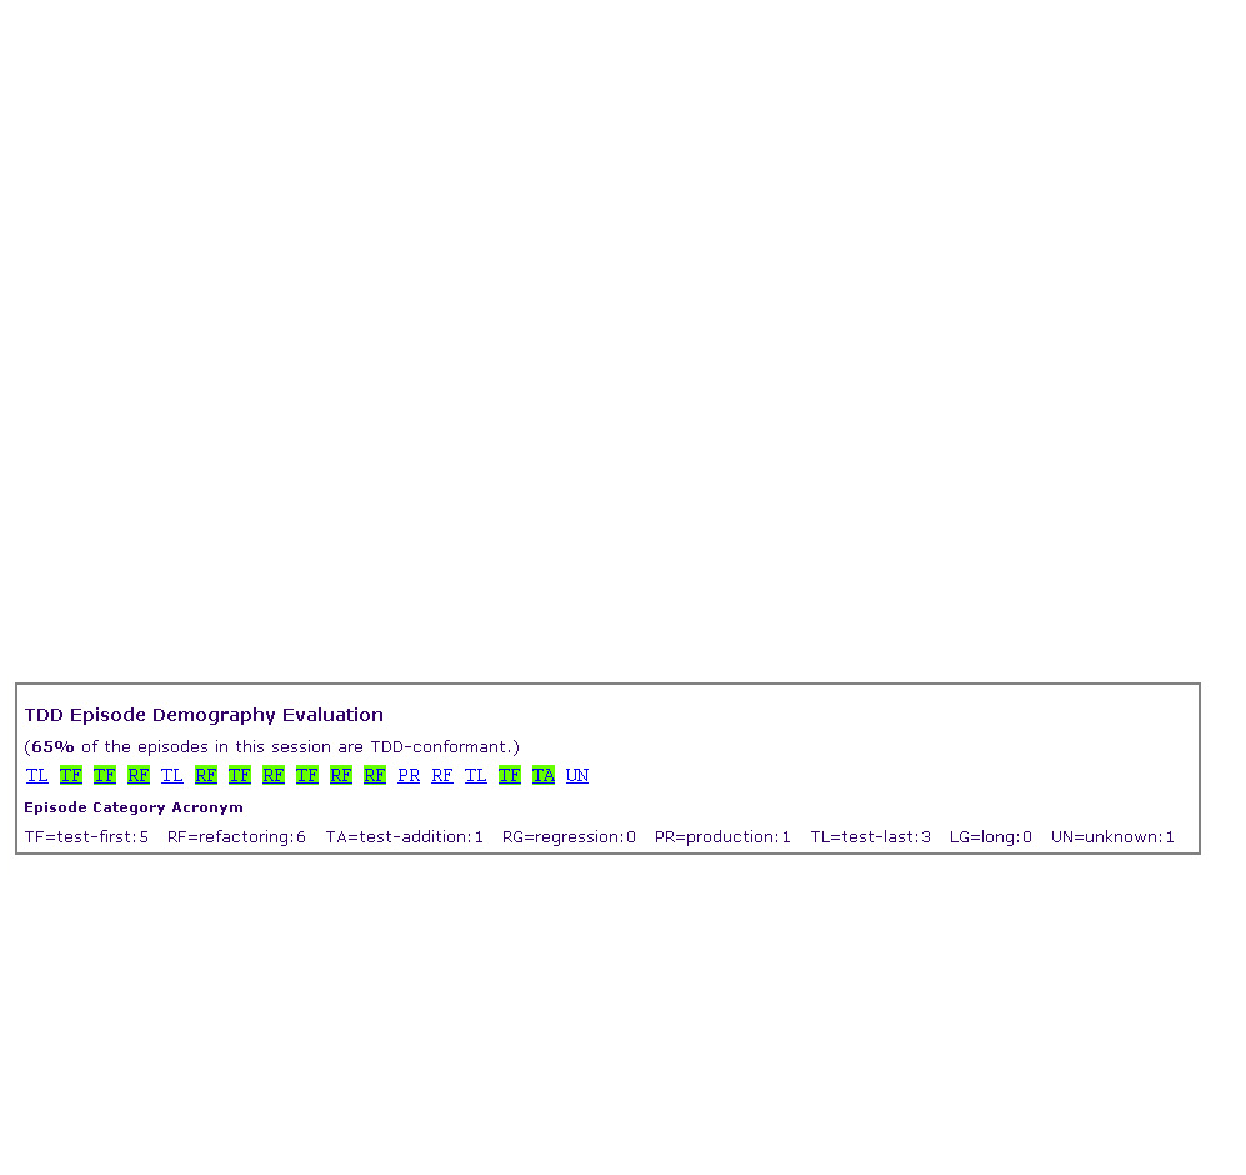
\includegraphics[width=1.0\textwidth]{figs/Zorro-DemographyAnalysis}
  \caption{TDD Episode Demography}
  \label{fig:Zorro-Demography}
\end{figure}
This analysis provides an overview of a TDD programming session, which is partitioned into 17 episodes, and 65\% of them are TDD compliant. Note that 
\begin{itemize}
\item each small box with a two-letter acronyms represents a single episode,
\item TDD-conformant episodes are shown in green. Non TDD-conformant episodes are transparent. 
\end{itemize}
For the TDD programming session illustrated in Figure \ref{fig:Zorro-Demography}, if Zorro was not used, the developer would falsely claim that he/she complied with TDD. In fact, as it turned out, the developer did not conform to the idealized TDD process all the time. According to Zorro's inference, 65\% percent of the episodes in this session are TDD-Conformant, and some episodes are ``test-last''. In addition to reporting the compliance of TDD, the ``TDD Episode Demography'' analysis can also be used to look for the development patterns. Episodes are ordered by time when they occurred. The researchers and developers can retrospectively review the development process for training or improvement. 

Besides typical analyses such as ``TDD Episode Demography'', I also implemented a group of telemetry analyses. The Software project telemetry \cite{csdl2-04-11,csdl2-06-05} was developed by Qin Zhang in the Collaborative Software Development Lab at the University of Hawaii. It can aggregate metrics data together to perform daily, weekly, or monthly analyses of the software metrics to support in-process software project management and decision makings. 
 
Some goals of this dissertation research are to assist the education, training, improvement, and empirical evaluations of TDD. Software project telemetry is an infrastructure that can be used by Zorro to pursue these goals. In Zorro, I have already defined telemetry streams including ``TDD percent of development time'', ``TDD percent of episodes'', ``development time ratio of test and production code'', ``size ratio of test and production code'', and so forth. Figure \ref{fig:Zorro-TDD-Coverage} is a weekly telemetry chart showing percentage of TDD development and test coverage.
\begin{figure}[htbp]
  \centering
  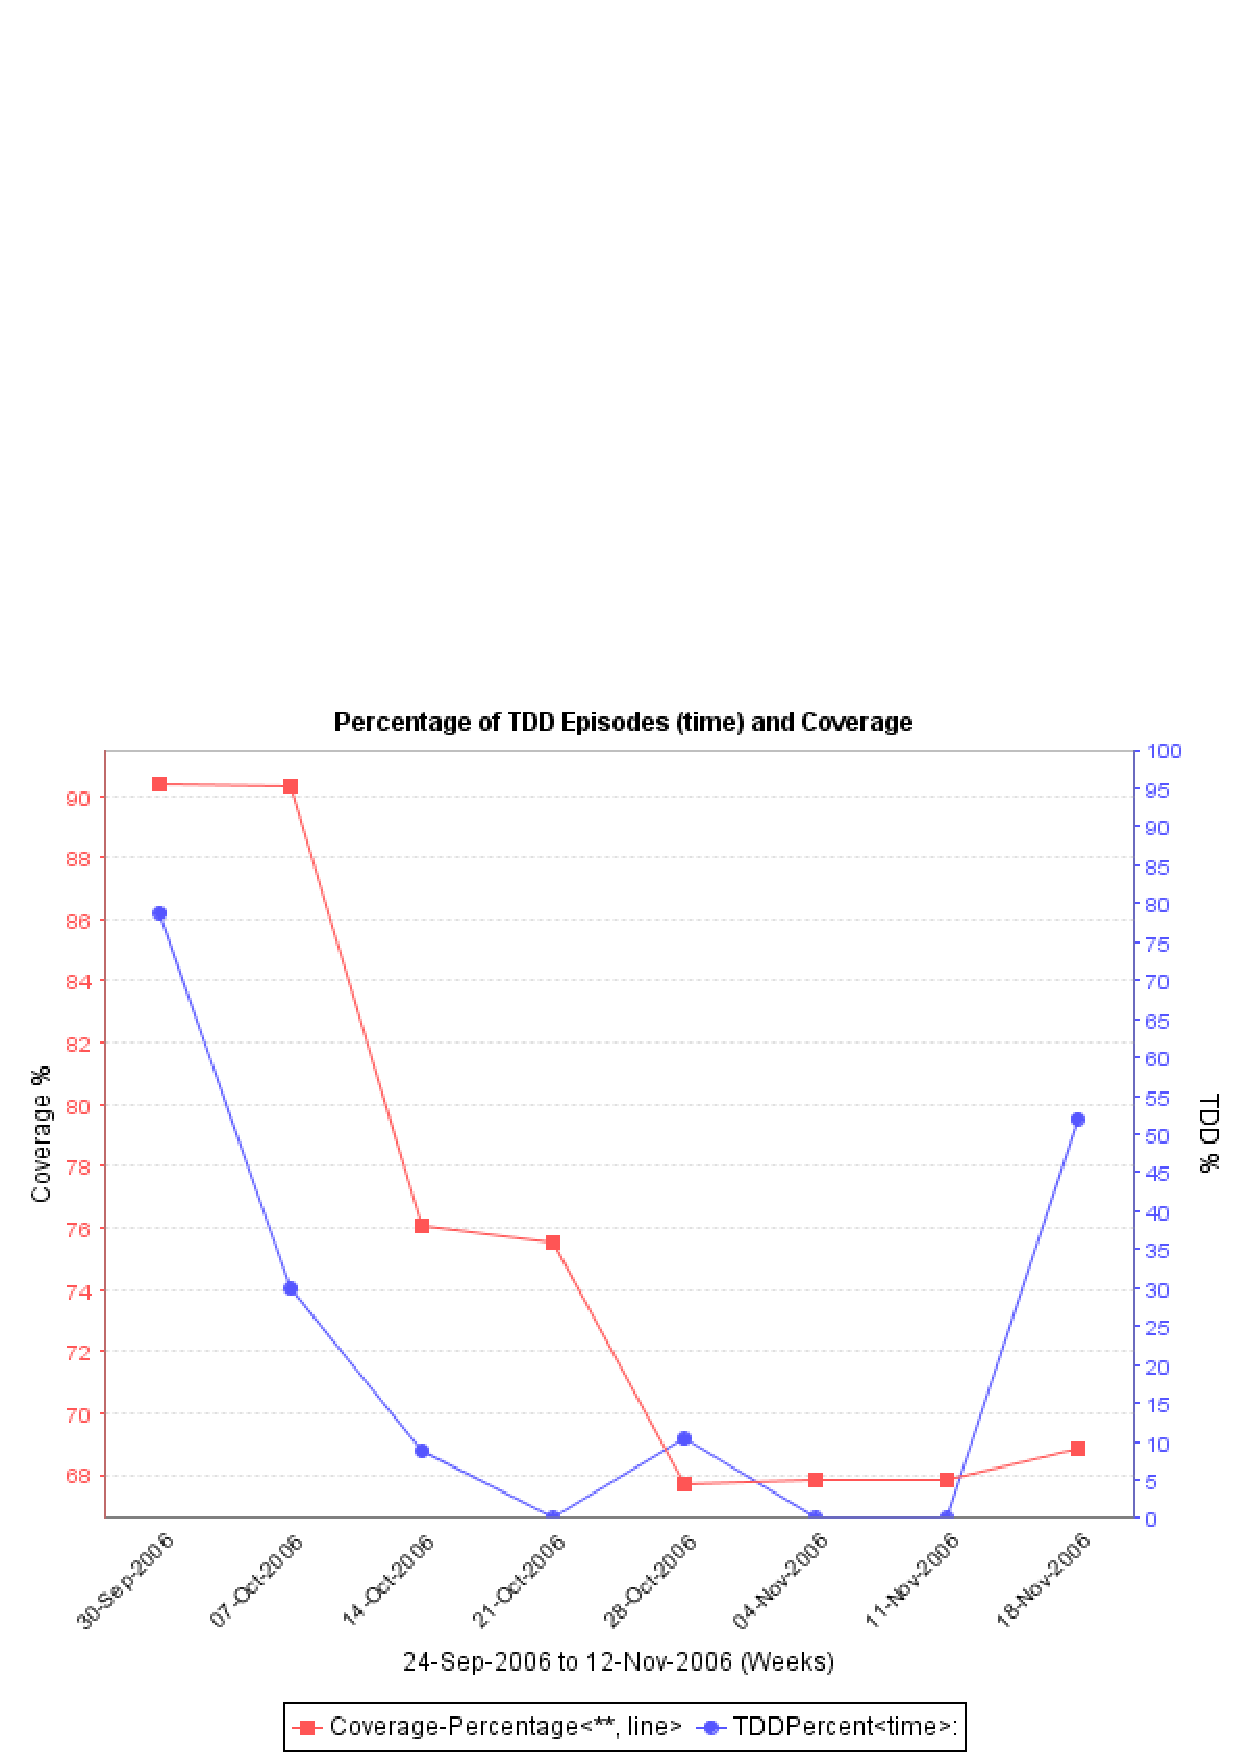
\includegraphics[width=1.0\textwidth]{figs/Zorro-TDD-Coverage}
  \caption{Proportion of TDD vs Test Coverage}
  \label{fig:Zorro-TDD-Coverage}
\end{figure}
From the week of Sep 30, 2006 to the week of Nov 18, 2006, I worked on the Zorro software system and implemented Zorro's web validation interface. I used TDD in my development. Due to the fact that testing web interfaces requires a lot of additional effort, my percent of TDD development dropped down significantly in that period. As a result, the test coverage of Zorro dropped from above 90\% to below 70\% over the course of eight weeks software development. 

The synergy of Zorro and telemetry allows practitioners and researchers to improve the practice and research of TDD with no additional overhead. Both systems are automated based on Hackystat's automatic software metrics collection with sensors attached to the development environment tools. 

\section{Research Statement}
In this dissertation, I created the Zorro software system to study the conformance of Test-Driven Development in practice with the aids of the Hackystat framework and the Software Development Stream Analysis (SDSA) framework that I have developed. The design of the Zorro software system is a combination of bottom-up and top-down methods. The development environment tools are instrumented by Hackystat sensors to collect software process and product metrics. A variety of software metrics are abstracted into development activities and then are merged together to form the time-series software development stream, which is then partitioned into small chunks named ``episode''. This portion is bottom-up. Given a software development method or low-level software process, the process description, guideline, and knowledge can be translated into a set of rules. The rules can be used to evaluate episodes partitioned from the software development stream. This portion is top-down.

The success of Zorro relies on the software metrics collection capability as well as the comprehension of TDD. The software metrics that are related to TDD must be collected. In the long run, it is important for the software development community to reach some kind of consensus on an appropriate definition (or definitions) for TDD. Until there is concrete experience from Zorro, this consensus is not feasible. The development of Zorro is thus iterative and progressive. Figure \ref{fig:Zorro-Timeline} illustrates the time line of this research project including a few milestones. 
\begin{figure}[htbp]
  \centering
  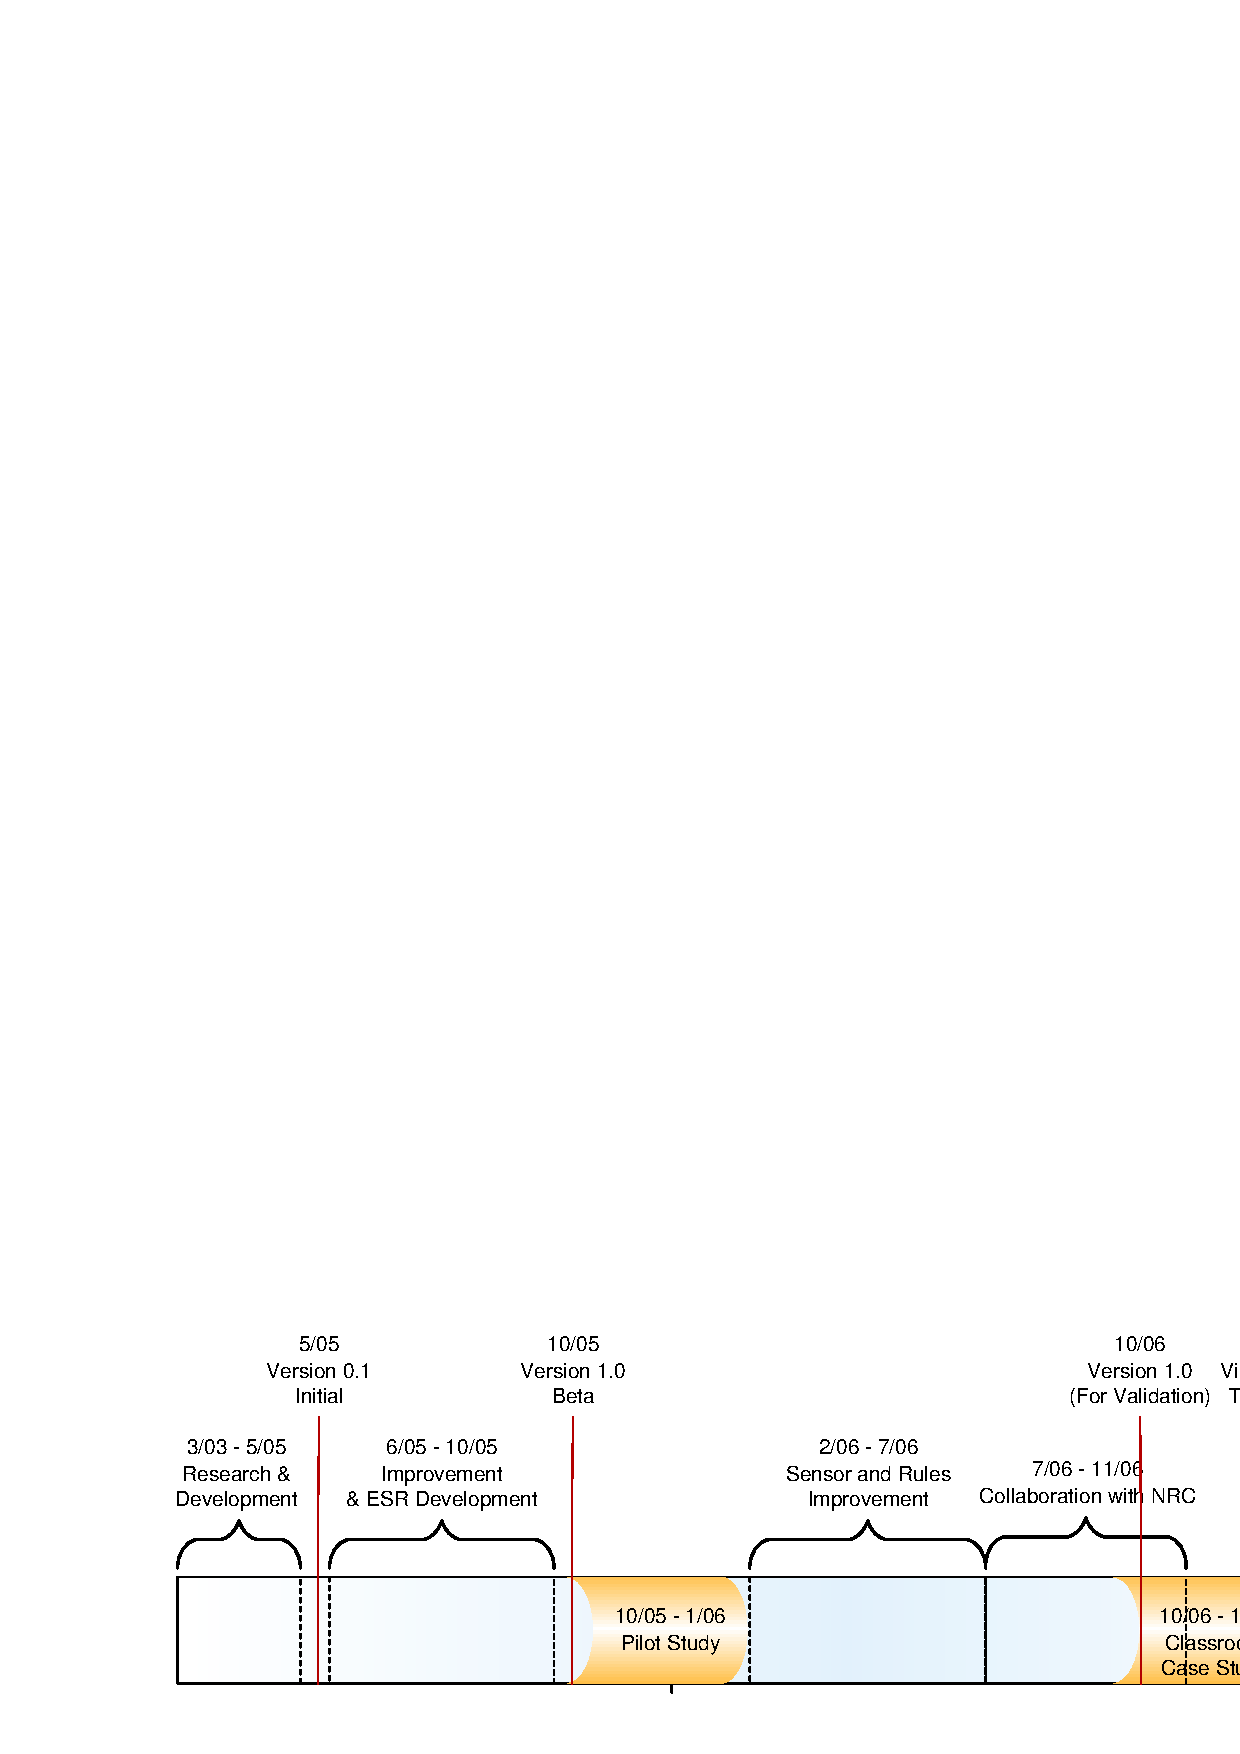
\includegraphics[width=1.0\textwidth]{figs/Visio-Zorro-TimeLine}
  \caption{Development Timeline of the Zorro Software System}
  \label{fig:Zorro-Timeline}
\end{figure}
I have conducted three empirical evaluations in my development process of Zorro to investigate whether Zorro can collect enough software metrics and how well it can infer TDD compliance. The Eclipse Screen Recorder (ESR, \cite{esr}), an Eclipse plug-in that can record development activities in the Eclipse IDE, was developed to assist the evaluations. ESR can capture Eclipse screen at the rate of 1 frame per second, and thus it provides high fidelity movies for the purpose of validation. The last empirical case study was conducted off-site in Norway to investigate what values Zorro can provide for researchers and project managers. 

\section{Empirical Evaluations}
\label{sec:introduction-evaluation}
Three longitudinal case studies --- a pilot study, a classroom case study, and an industrial case study were conducted to empirically validate the Zorro software system in this dissertation research. The primary goal of these studies was to validate Zorro's software metrics collection as well as TDD inference abilities. The secondary goal was to investigate how useful Zorro would be. An additional goal was to investigate how the metrics collection and inference rules can be improved. 

\begin{comment}
The software development processes in both studies were instrumented by the Eclipse Screen Recorder (ESR) \cite{esr}, an Eclipse plug-in that can record the software development process in the Eclipse IDE. The videos recorded by ESR were analyzed to validate Zorro's data collection and TDD inference. 

The goal of the first two studies was to evaluate and improve Zorro's software metrics collection and TDD inference capability in academic settings. 

tune the sensor and inference rules. The industrial case study was an attempt to deploy Zorro in the real TDD development situations. The primary goal was to explore how Zorro can assist project managers and researchers gaining insights of TDD.
\end{comment}

\subsection{Pilot Study}
After researching related work on TDD and stream analysis techniques, I designed and implemented the Zorro software system based upon my observation and analysis of TDD development patterns. By the Spring 2005, I had solved all the difficulties of metrics collection in the Eclipse IDE as a pilot, implemented the SDSA framework, and developed the first set of TDD recognition rules. 

I refined the initial version of Zorro in the Summer 2005, and conducted a pilot validation study in the Fall 2005. Six experienced Java programmers participated in this study. Each participant developed a implementation of the stack data structure (Appendix \ref{app:PilotStudyMaterial}) using TDD in the Eclipse IDE, which was instrumented by the Hackystat Eclipse sensor. I compared Zorro's inference to an independently collected source regarding their development behaviors. 

One approach to independent data collection would be to have an observer watching developers as they programmed, taking notes as to what development behavior they are conducting and whether they are pertaining to TDD or not. I considered this but discarded it as unworkable: given the rapidity of development activities in TDD, it would be very hard for an observer to notate all of the TDD-related development activities that can occur literally within seconds of each other. Therefore, I took another approach by developing the Eclipse Screen Recorder \cite{esr}. The ESR generates a QuickTime movie containing time-stamped screen shots of the Eclipse Window at the regular intervals. One frame/second was found to be sufficient for validation, generating file sizes of approximately 7-8 MB per hour of video. The QuickTime movie created by ESR provides a visual record of development behaviors that can be manually compared to the Zorro analysis using the timestamps for validation purpose. Figure \ref{fig:ESR-Video} is a screen copy showing the recorded development process movie played in the QuickTime Pro software \cite{QuickTime}.
\begin{figure}[htbp]
  \centering
  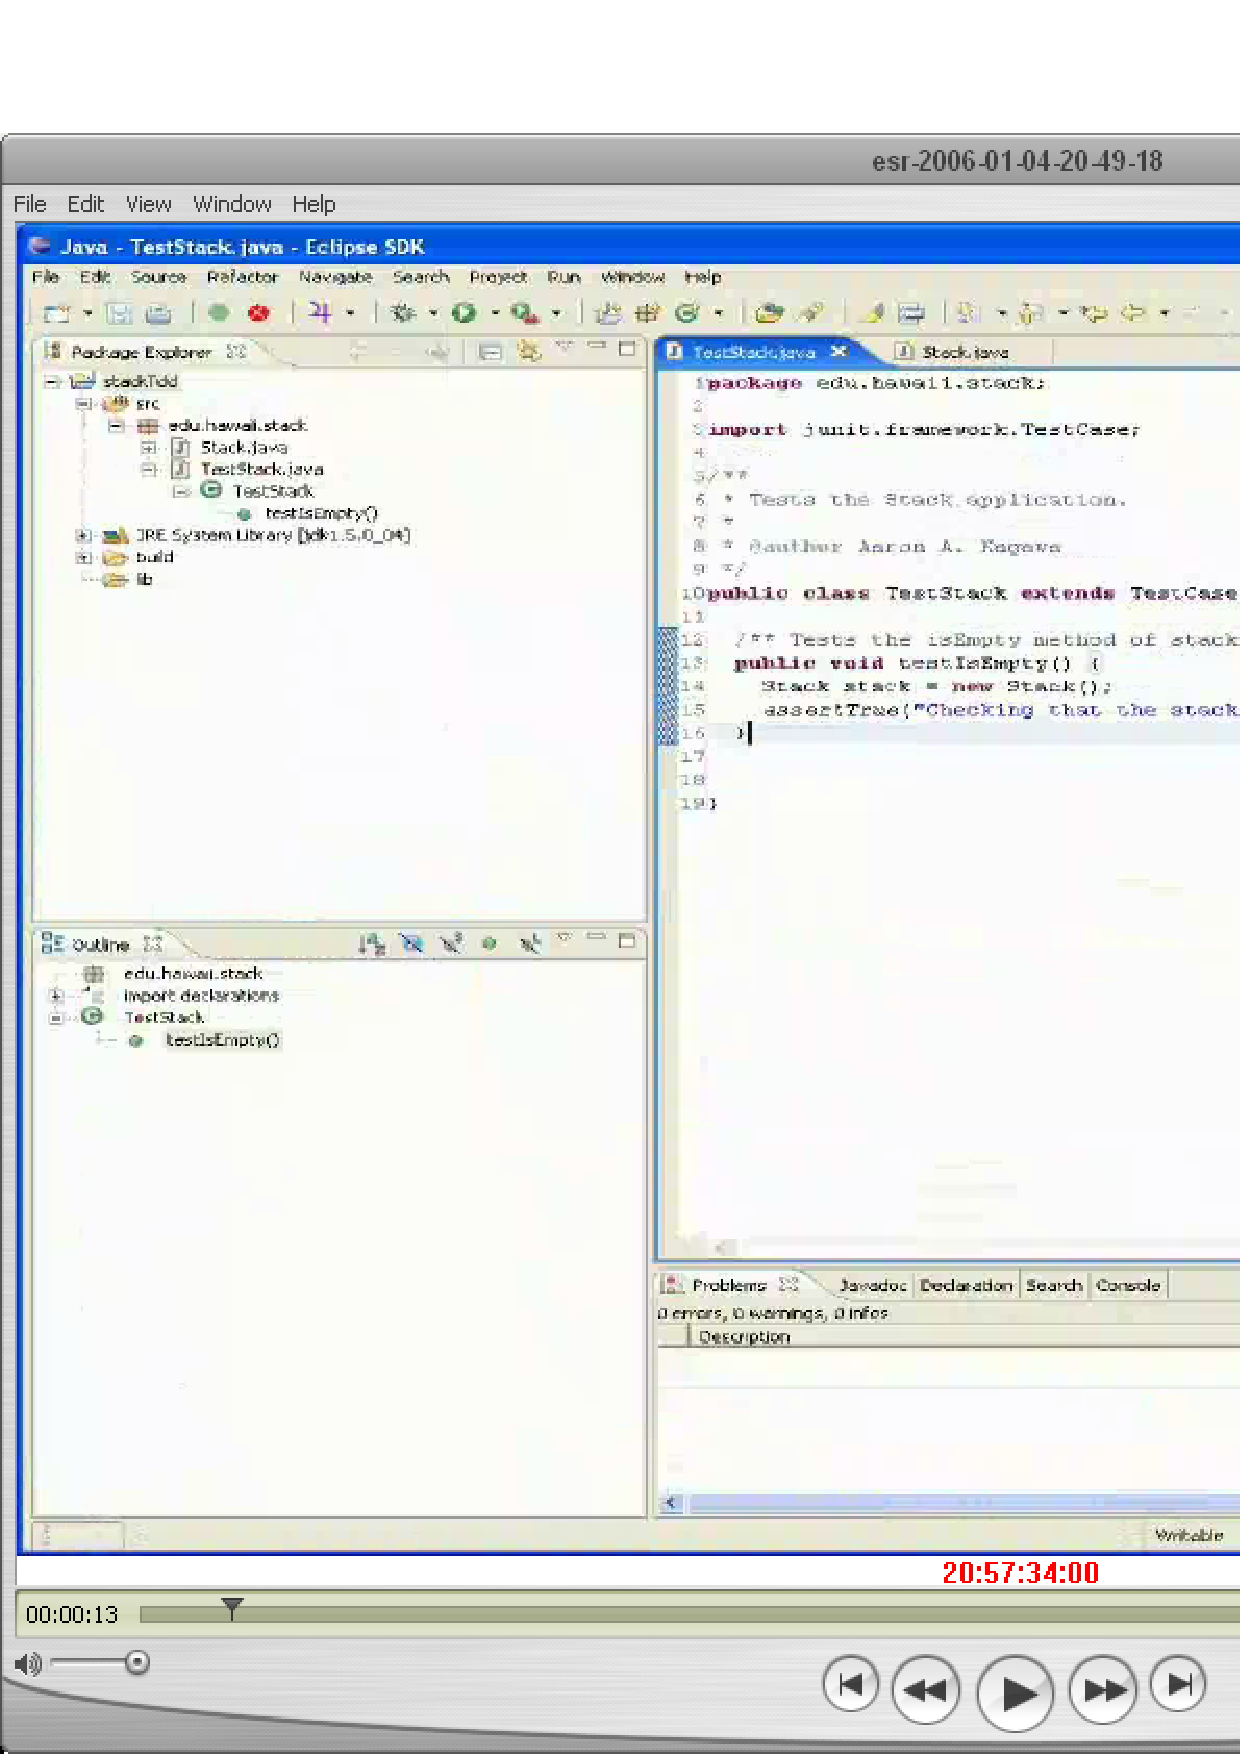
\includegraphics[width=1.0\textwidth]{figs/ESR-Video}
  \caption{Analysis of QuickTime Video}
  \label{fig:ESR-Video}
\end{figure}

The participants spent 28 to 66 minutes on the programming task. Zorro partitioned the overall development efforts into 92 episodes, out of which 86 were classifiable; 6 were unclassifiable. It classified 76 out of 86 episodes correctly resulting in classification accuracy rate 88.4\%.

The pilot study showed that Zorro is promising at inferring high-level development behaviors with low-level development activities collected as software metrics at least in a simple environment setting. The pilot study also showed that the metrics collection missed some information that led to inference errors. 

In the Spring 2006, I improved the Hackystat Eclipse sensor for metrics collection, and refactored Zorro's inference rules. In the Summer 2006, under the suggestion of Dr. Philip Johnson, I went to National Research Council of Canada (C-NRC), where I collaborated with Dr. Hakan Erdogmus, a senior agile process researcher who pioneered the idea of automated TDD conformance inference. The collaborative research at the C-NRC and the follow-up collaboration in the Fall 2006 resulted in a classroom case study and an industrial case study in the Spring 2007. 

\subsection{Classroom Case Study}
I, the author of Zorro, compared the recorded movies with Zorro's inference to validate Zorro's metrics collection and TDD development inference in the pilot study. I could be biased both at judging what software metrics are necessary, as well as at inferring development behaviors from the observed activities in the ESR movies. One man's subjective judgment, especially the one from author himself or herself, perhaps is not a valid measure in a case study \cite{Yin:03}. This is notably called ``construct validity'' problem according to \cite{Yin:03}. Using multiple data sources, establishing the chain of evidence, and having key informants review draft case study report are three viable tactics that a researcher can use to avoid the construct validity problem. Thus, in the Fall 2006, I developed a web interface to collect participant's comments, the third data source. 

In the Fall 2006, I conducted the classroom case study in the software engineering classes at the University of Hawaii. The  experimental design of this study is very close to the pilot study. Participants also developed using TDD in the Eclipse IDE with the instrumentations of the Hackystat Eclipse sensor and ESR. The differences were that the Hackystat Eclipse sensor was more robust and the new problem (Bowling Score Keeper at Appendix \ref{app:UserStoriesBSK}) was much harder than the stack data structure (Appendix \ref{app:PilotStudyMaterial}). 

Eleven students from the software engineering classes voluntarily participated in this study. The participants developed in TDD for 90 minutes, followed by a 10 minute interview and a 20 minutes Zorro inference validation session. In the interview, I asked them questions regarding their opinions on unit testing and Test-Driven Development. A digital voice recorder was used in the interview and in the following validation session for their verbal comments.

The classroom case study data analysis supported the claim that  Zorro's metrics collection is as good as ESR, if it is not better. Zorro's TDD compliance inference has two steps. It infers development behaviors in episode first, and then uses the inferred results and context to reason the conformance of TDD. The video analysis validated that Zorro inferred episode development behaviors with 70.1\% accuracy and TDD compliance with 89.1\% accuracy. The third data source, cross-validation with participant comments, is only slightly different from my video observation analysis. 

The participant interview analysis suggested that unit testing is good at yielding high quality software but majority of participants (7 out of 10) admitted that they did not test enough. Perhaps TDD should be used to improve both developers' confidence and software quality. The data analysis also suggested that TDD is hard to do although half of participants like to develop software using TDD in the future. Therefore, providing a tool such as Zorro to assist practice of TDD has the potential to help beginners. The usefulness evaluation conducted in this study suggested that some of Zorro's TDD analyses are useful for this purpose. 

\subsection{Industrial Case Study}
On one hand, I planned the classroom case study for an extended validation after the pilot study. On another hand, I worked with Dr. Philip Johnson and Dr. Hakan Erdogmus to solicit the collaboration with other researchers and practitioners who are also interested in empirical study of TDD. The Zorro demo \cite{ZorroDemo:06} was developed to demonstrate how Zorro works and what analyses it provides. This effort led to collaboration with Dr. Geir Hanssen and Dr. Tor Erlend F{\ae}gri from SINTEF ICT of Norway. They are performing research on the effectiveness of TDD, in contrast to Test-Last Development, the opposite side of TDD. They found that collecting the information about TDD is very hard and Zorro has the potential to provide higher quality information about TDD.

A European software company that provides a packaged software product for marketing and customer surveys \cite{Hanssen:06} is the participant of this industrial case study. However, the development tool is Visual Studio .NET Team Edition and the programming language is C\#. We rapidly developed a Zorro compatible Visual Studio sensor for this industrial case study. A Hackystat server is installed on a Windows 2000 server provided by the company. I remotely managed the server for this industrial case study. Out of 20 participants, 12 were in the TDD project and the remaining 8 were in the non-TDD project. Unfortunately, the participation in this study was very low. As to my report written at the end of March 2007, 25\% of developers installed the sensor and collected development data,  25\% of developers installed the sensor but did not update it as requested, 25\% of developers installed the sensor but the sensor did not send any data to the server after a pilot, and the rest 25\% of developers did not install the sensor according to my 
observation of the Hackystat server status. The project manager indicated that Zorro's inferred development behaviors did not agree with what developers actually did, but provided no detailed information. It turned out that it is much harder to have industry participants install the sensor, and it is also hard to relate collected data to actual development behaviors, particularly if the study had to be conducted remotely. However, Dr. Geir Hanssen and Tor Erlend F{\ae}gri have expressed interests to continue using Zorro in the future studies. This case study served as a pilot test only.  

\section{Contributions}

My contributions include the SDSA framework, the Zorro software system, and the systematic empirical evaluation of Zorro:
\begin{enumerate}
\item \textbf{SDSA Framework}

The Software development is a very complicated process including a series of continuous development activities, yet not independent of each other. The SDSA framework abstracts continuous, interwoven development activities collected by Hackystat sensors in a programming session into a software development stream. The software development stream is a linear, time-series data structure. 

A development stream can be partitioned by SDSA using tokenizers into episodes, another abstract data type representing a micro-iteration of a software process. Tokenizers are expandable and selectable. A different set of tokenizers can be applied according to the studied software process.

The SDSA framework characterizes development behaviors in episodes using JESS, a rule-based system in Java. A classifier interface is provided in SDSA to flexibly supply inference rules. Moreover, the rules can be changed on the fly. 

In my thesis research, I instantiated the SDSA framework on Test-Driven Development (TDD), and the system resulting from this work is the Zorro software system that can automatically infer the development behaviors and the compliance of TDD. This research work demonstrated that the SDSA framework has the potential to be useful for researching other low-level software processes. 

\item \textbf{Automated Recognition of TDD with Zorro}

Zorro recognizes TDD automatically with the software metrics collected by Hackystat sensors in the IDEs. The contributions of Zorro's implementation include the enhanced Eclipse and Visual Studio .NET sensors, a suite of TDD recognition rules, and many useful analyses for understanding TDD in practice.

The Eclipse and Visual Studio .NET Team Edition are two IDEs that are Zorro compatible. The sensors of these two IDEs collect a variety of process metrics such as editing, refactoring, testing, compilation, and so on. Many useful product metrics such as methods, statements, test cases, and assertions are collected too. The progressive changes of software product metrics are very useful information for software engineering research.

The recognition rules are from the descriptions of many well-known TDD practitioners including Beck \cite{Beck:03}, Doshi \cite{TDDQuickReference}, and Erdogmus, and my grounded observation of TDD in practice. 

Many analyses were developed to display Zorro's inference processes and results, report different aspects of TDD such as episode duration distribution. The TDD telemetry streams were developed to support the in-process decision makings for software project management.  

\item \textbf{Empirical Evaluations}

My contribution to the empirical evaluations are:
\begin{enumerate}
\item ESR \cite{esr}, a software system that can record Eclipse usage; 
\item The availability of the Zorro software system for use by other researchers under an open source license;

\item The experimental method exemplified by the case studies, which shows how to conduct research on TDD that does not suffer from the process conformance problem;

\item The actual results of the case studies, which show (i) the Zorro can identify TDD, that (ii) users found Zorro analyses to be useful in certain cases and not in others, and (iii) that industrial case studies on TDD are more difficult than classroom case studies, as it is more difficult to get developers to install sensors, and more difficult to relate data back to their development.

\end{enumerate}
\end{enumerate}

\section{Dissertation Structure}

This thesis is organized into the following chapters. 

\begin{itemize}
\item Chapter 1 introduces the TDD challenges and the motivation of this research. 
\item Chapter 2 presents the related research work. 
\item Chapter 3 describes the SDSA framework in details.
\item Chapter 4 describes the Zorro software system in details.
\item Chapter 5 briefs the research questions and methodology of this dissertation. 
\item Chapter 6 reports the pilot study data analysis in details.  
\item Chapter 7 reports the classroom case study data analysis in details.
\item Chapter 8 reports the industrial case study conducted off-site.
\item Chapter 9 synthesizes the results from the empirical case studies, presents
the conclusions of this research, and discusses the future work.
\end{itemize}

\begin{comment}

The software development is a highly cognitive process in which developers continuously interact with development environment tools to produce the software artifacts following a certain process. 

Software metrics are great assets out of research work in the software engineering discipline. The typical use of software metrics is through the Goal-Question-Metric (GQM) paradigm where the software metrics are used as the measure to high-level questions and goals.  A significant drawback of the GQM is that software metrics are not always possible to be collected, or can be collect in high cost. 
\end{comment}

%%%%%%%%%%%%%%%%%%%%%%%%%%%%%%%%%%%%%%%%%%%%%%%%%%%%%%%%%%%%%%%%%%%%%%%%%%%%
%% Start of the old introduction
\begin{comment}
Throughout the history of software engineering, much effort has been put on the description and understanding of high-level software processes. The waterfall model, the very first software process, has contributed to the success of many large software systems. High-level software processes divide the software development process into phases, where each phase lasts from a few days to several months \cite{Pfleeger:01,Pressman:03}. For example, the requirements analysis phase may last months before the design phase starts. Recently, increasing effort has been put on low-level software processes \cite{Larman:03,AgileAlliance}, in which a phase may last several minutes to a few hours only. Each phase defines how developers and development team should carry on the work on daily basis. The Personal Software Process (PSP) \cite{Humphrey:99} and Extreme Programming (XP) \cite{Jeffries:00,Beck:00,XP96} are two examples of a low-level software process. Although proven to be useful in improving software quality\cite{Ferguson:97,Kamatar:00,MicrosoftTSP,Janzen:05}, low-level software process are hard to execute correctly and repeatedly. In order to improve the quality of practice and research of low-level software process, there must be some supporting tools. In my dissertation research, I focus on one low-level software process, the called Test-Driven Development (TDD) \cite{Beck:03}, and I developed Zorro software system to study it.

Test-Driven Development (TDD) is an innovative one of the practices of Extreme Programming. In TDD, the software development process is iterative and incremental \cite{Larman:03}. There is only one task to accomplish in an iteration. In a particular iteration, a unit test of the task is created first followed by production code implementation.  TDD is built on the foundation of the XUnit framework \cite{XUnit}, which has been ported to more than 30 languages. Unit testing has become a de facto standard in the software industry. TDD is widely adopted by software professionals. An informal survey \cite{UnitTestingPoll:06} conducted by Method and Survey magazine found that 46\% of the studied software organizations perform unit testing informally, 41\% of the studied organizations document their unit test cases, and 14\% of the studied organizations use the TDD approach.

``Clean code that works''\cite{Beck:03} is the goal of Test-Driven Development. To achieve this goal, TDD summarizes its software development process as two basic rules: ``(1) Write new code only if an automated test has failed; (2) Eliminate duplication.''  Kent Beck, the pioneer of Test-Driven Development, stated that there is an implicit order to software development using TDD \cite{Beck:03}: 
\begin{enumerate}
\item Red - Write a little test that does not work, and perhaps does not even
  compile at first.
\item Green - Make the test work quickly, committing whatever sins are
  necessary in the process.  
\item Refactor - Eliminate all the duplication created by merely getting
  the test to work.  
\end{enumerate}
At first glimpse, TDD seems easy, but in fact, it is a very hard and difficult low-level software process that requires much discipline to carry out correctly. First, software developers are not typically educated to write unit tests for the program they develop. Therefore, in a lot of cases, software systems are not designed for easy testing. Consequently, developers often find it is hard for them to write testing code at all, much less write testing code prior to implementation. Second, following the red/green/refactor software development pattern requires a lot of effort. In TDD, software developers must continuously remain in the mindset of test-first, which is initially counter-intuitive to many of them \cite{Beck:01,Wang:04}. So they often apply it differently according to their own experience level and understanding \cite{Beck:01}.

TDD is gradually becoming a standard well accepted for software development in industry, and yet there are problems in testability and differences in understanding of this methodology. Not surprisingly, the immaturity of TDD causes problems. There are many important research questions regarding software development using TDD. For example, how do we know software developers will faithfully commit to the highly disciplined TDD practice? Will developers slip away from TDD? When does it pay off to use TDD, and when does it not pay off? One thing is clear: these questions cannot be answered accurately without good software process measurement. However, Janzen and Saiedian \cite{Janzen:05} stated that measuring the use of a software development methodology is hard. They claimed it is so hard to do accurately that published data on the level of TDD adoption in industry is either indirect or inaccurate \cite{Janzen:05,UnitTestingPoll:06}.  Fortunately, as my initial case study demonstrates, measuring the use of certain software development methods is becoming feasible with the emergence of technologies such as the Hackystat system \cite{Hackystat:06,csdl2-04-11,csdl2-04-22,csdl2-03-12}, an in-process software metrics collection and analysis framework.

As part of my dissertation research, I developed a software system called Zorro (Figure \ref{fig:ZorroInfrastructure}) on top of Hackystat to infer TDD development behaviors using low-level software development activity data collected by Hackystat Eclipse Sensor.  Zorro recognizes and evaluates TDD patterns using rule-based system support and the software development stream analysis (SDSA) framework. SDSA is a three-stage analysis technique that brings the Hackystat framework and Zorro system together. First, it merges software development activities and in-process metric data together to create a ``software development stream'', a sequential stream of low-level software development activities. Second, SDSA includes a tokenization subsystem that divides a single sequential stream of low-level software development activities into collections of events called ``software development episodes''. Third, the JESS \cite{Friedman-Hill:03} rule-based system recognizes and classifies these episodes according to the classification schema.  SDSA binds these three components together to assist the measurement of software development methods and low-level software process.
\begin{figure}[htbp]
  \centering
  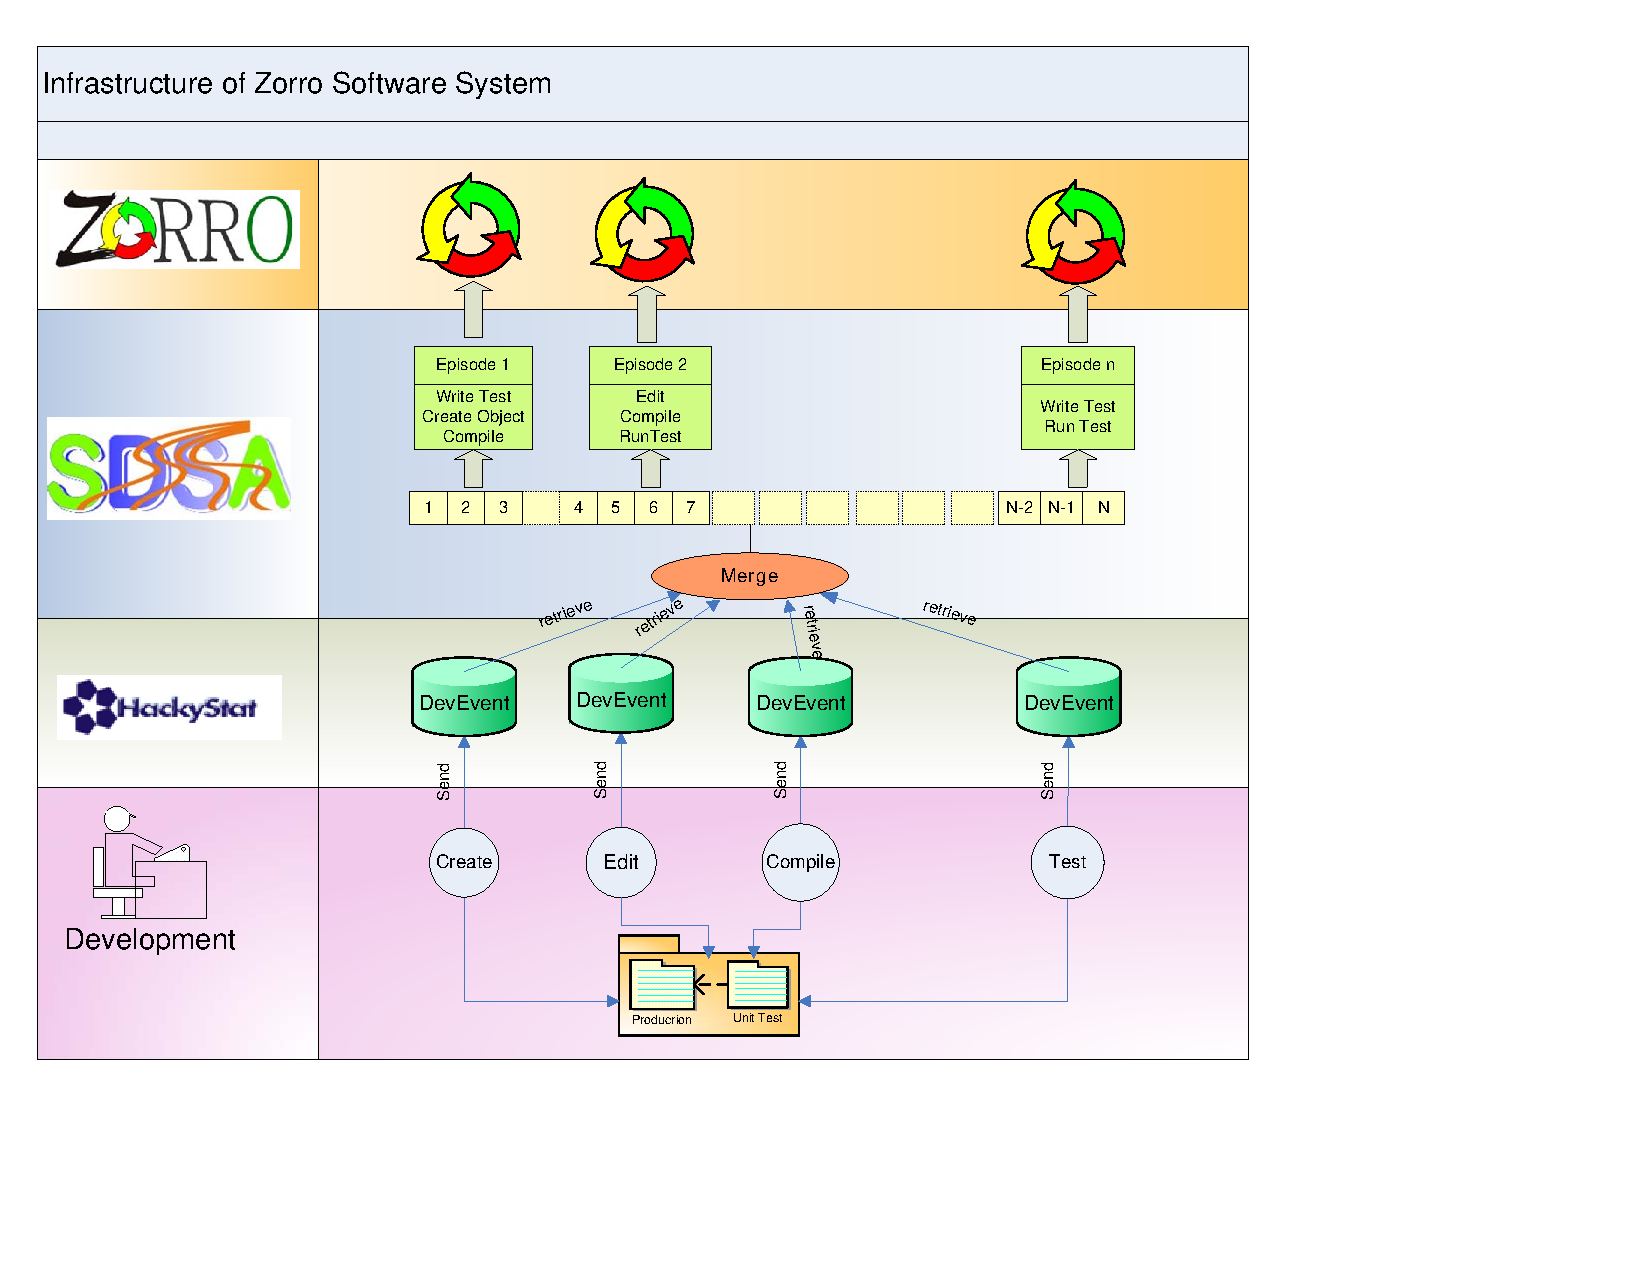
\includegraphics[width=0.9\textwidth]{figs/Visio-ZorroInfrastructure}
  \caption{Zorro Infrastructure}
  \label{fig:ZorroInfrastructure}
\end{figure}

With the capabilities provided by SDSA, I defined a set of specific rules for TDD in Zorro according to Beck \cite{Beck:01,Beck:03} and others who have described the practices of TDD. Zorro uses a two-step procedure to measure and evaluate the compliance of the developer's behaviors with the practices of TDD.  First, Zorro recognizes and classifies the episodes independently according to the classification schema. Second, Zorro evaluates the internal structure as well as the context of the episodes to deduce whether an episode is TDD conformant or not.
\end{comment}